\section{Matroidok összege, k-matroid-metszet probléma és bonyolultsága}

\[
	\begin{rcases}
		M_1=(E,F_1), \\
		M_2=(E,F_2)
	\end{rcases}
	\Rightarrow
	M_1 \vee M_2  = (E,F'), X \in F' \Leftrightarrow X_1, X_2
	\begin{cases}
		X=X_1 \cup X_2 \\
		X_1 \in F_1    \\
		X_2 \in F_2
	\end{cases}
\]

Tehát a matroid összegében azon elemek jelenek meg amelyek előállnak $F_1$ és
$F_2$--beli elemek uniójáként.

\vspace{0.4cm}
\emph{Matroidok összege is matroid.}
\vspace{0.4cm}

A bizonyitáshoz ellenőrizzük a függetlenségi axiómákat. F$1$ és F$2$
nyilvánvaló, tehát csak F$3$--at látjuk be indirekt. Tegyük fel, hogy nem igaz, $X,Y \in F'$
és $|X|>|Y|$, de nem létezik $x \in X-Y$, hogy $Y+x \in F$. $X$ és $Y$
halmazokank mindig létezik $X=X_1 \cup X_2$ és $Y=Y_1
	\cup Y_2 ~(X_1, Y_1 \in F_1, X_2, Y_2 \in F_2)$ felbontása.

\begin{figure}[htbp]
	\centering
	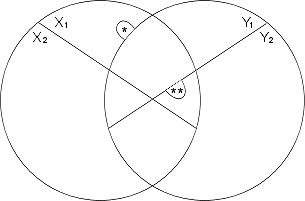
\includegraphics[width=0.4\linewidth]{./kepek/matroidosszeg.png}
	\caption{Matroid összeg bizonyitás}\label{fig:Unif}
\end{figure}

Válasszunk egy olyan felbontást, hogy a részhalmazok diszjunktak legyenek,
$|X_1|>|Y_1|$ és az $|X_1 \cap Y_2|+|X_2+Y_1|$ összeg minimális értéket vegyen
fel. Ekkor $M_1$ matroidra alkalmazva az F$3$--at: létezik $x \in X_1-Y_1$,
hogy $Y_1+x \in F_1$.

Ha $x \not \in Y_2$ akkor $x+Y $ benne van az összegben $(\in F')$, ami
ellentmondana az indukciós feltevésünknek. Tehát $x \in Y_2$, amiből következik,
hogy létezik egy másik felbontás $Y=(Y_1+x) \cup (Y_2 -x)=Y_1^* \cup Y_2^*$.
Erre viszont a $|X_1\cap Y_2^*|+|X_2 \cap Y_1^*|$ összeg egyel kevesebb, ami
elentmond annak, hogy mi már a lehető legkisebbet választottuk korábban. Tehát a
feltvésünk hamis volt, F$3$ igaz.

\vspace{0.4cm}
\emph{$M=(E,F)$ matroid szabadmatroid, ha bármely részhalmaza független.}

\subsection{\texorpdfstring{Matroid metszet probléma -- MMP\textsubscript{$k$}}
	{Matroid metszet probléma -- MMPk}}

Adott $k$ darab matroid közös alaphalmazon: $M_i=(E,F_i)_{i=\overline{1,k}}$. A
kérédés amire keressük a választ, hogy létezik e $p \in \mathbb{N}$ konstansra
$p$ méretű halmaz $\cap F_i$--ben. Az eredmény nem minden esetben lesz matroid.

\vspace{0.4cm}
MMP$_2 \in $P.
\vspace{0.4cm}

A bizonyitáshoz induljunk ki egy adott $M_1=(E,F_1)$ és $M_2=(E,F_2)$ matroid
párból és legyen $p$ a halmazrendszerek metszetébben keresett halmazok mérete.
Ha $p>min(r_1, r_2)$ akkor a válasz nem, ilyen méretű halmaz nem létezik.
Másképpen csonkoljuk a két matroidot amig rangjuk min$(r_1,r_2, p)$--re nem
csökken:

\[ \begin{rcases}
		M=(E,F) \mbox{ egy p rangú matroid} \\
		0 \leq k \leq p                     \\
		p \geq 1
	\end{rcases} \parbox[t]{5.5cm}
	{$F' = \left\{ X \subseteq E: X \in F, |X| \leq k \right\}$
		$(E,F')~M$ csonkolat matroidja} \]

Ezzel a problémát redukáltuk a közös bázis megkeresésére. $r_1=r_2=p$--re a
válasz akkor és csak akkor igenlő ha létezik ilyen méretű közös bázis, azaz ha
$M_1 \vee M_2^*=(E,2^E)$ szabad matroid.

$\Rightarrow$ Ha $M_1$ és $M_2$--nek van egy közös $B$ bázisa, akkor $M^*$--ban
$E-B$ bázis. Az $E=B \cup (E-B)$ egy felbontása az összegnek, azaz az összegben
$E$ független, tehát $M_1 \vee M_2^*$ szabadmatroid.

$\Leftarrow$ Legyen $E=C \cup D$ egy olyan felbontása a szabadmatroidnak, hogy
$C \in F_1$ és $D \in F_2^*$. Ekkor:
\[|E| \leq |C| + |D| = r_1(C) + r_2^*(D) \leq r_1(E)+r_2^*(E) = r_1(E) + |E| - r_2(E)=|E|. \]

Mivel $C$ és $D$--t diszjunkt halmazoknak választottuk, $C$ közös bázisa az $M_1$ és
$M_2$ matroidnak.

\subsection{Bonyolultság}

MMP\textsubscript{$k$} bonyolultsága ha $k \geq 3$--ra NP teljes. A feladat
NP--beli mert a $p$ elembeli halmaz közös tanú a két halmazrendszerre.

Az NP teljességhez figyeljük meg, hogy MMP\textsubscript{$3$} visszavezethető
Hamilton út keresésére (amiről tudjuk, hogy egy NP teljes probléma). Legyen $G$
irányított gráfban $u$ és $v$ között Hamilton út keresés:

\[
	\begin{cases}
		\begin{rcases}
			M_1=(E,F_1)   \\
			X \subseteq E \\
			X \in F_1
		\end{rcases} & \Leftrightarrow \parbox[t]{10cm} {$X$ részgráfban minden pont
		befoka legfejlebb egy, és az $u$ befoka nulla.}                              \\
		\begin{rcases}
			M_2=(E,F_2)   \\
			X \subseteq E \\
			X \in F_2
		\end{rcases} & \Leftrightarrow \parbox[t]{10cm} {$X$ részgráfban minden pont
			kifoka kisebb vagy egyenlő eggyel egy és a $v$ kifoka nulla.}
	\end{cases}
\]

Ekkor M$_3$  a gráf körmatroidja, és M$_1$, M$_2$, M$_3$ közös $|V|-1$ elemű
bázisai $G$ gráf irányított Hamilton útjai.

\vspace{0.4cm}
\emph{MMP$_k$, ha $k>3$ NP teljes.}
A bizonyitáshoz az imént konstruált struktúrához vegyünk hozzá $k-3$ darab
szabad matroidot.
